\graphicspath{ {./img/2_Theory/} }


\chapter{Fotogrametria. Wprowadzenie teoretyczne}

Fotogrametria - dziedzina nauki, rodzaj sztuki i technologia mająca na celu wyznaczanie informacji i odtwarzanie kształtów jednego lub więcej obiektów fizycznych na podstawie zdjęć obiektów.
Fotogrametrię można podizielić na dwa rodzaje: płaską i przestrzenną. Fotogrametria płaska wymaga co najmniej jednego zdjęcia i jej wynikiem jest charakterystyka obiektu w płaszczyźnie. Fotogrametria przestrzenna wymaga dwóch lub więcej zdjęć, jest używana do odtwarzania obiektów w przestrzeni trójwymiarowej.

W tej pracy stosowana jest wyłącznie fotogrametria przestrzenna.

Pozwala ona wyznaczyć takie charakterystyki jak:
\begin{itemize}
   \item kszałt
   \item rozmiar
   \item położenie wzajemne w przestrzeni
   \item kolor i teksturę
\end{itemize}

Dodatkowo technologia fotogrametrii pozwala na wyznaczenie położenia kamery (obserwatora) w chwili robienia zdjęcia fotogrametrycznego.
Położenie kamery w przestrzeni trójwymiarowej jest wyznaczane na podstawie bazy sceny i wybranego zdjęcia zawierającego całość lub część sceny.

\textbf{Cecha}, punkt kluczowy --- element charakterystyczny obiektu wyróżniający się na tyle, aby można było zidentyfikować ten sam element na zdjęciu z innego ujęcia.

Pojęcie \textbf{sceny fotogrametrycznej}, często wykorzystywane w tej rozprawie, oznacza zbiór statycznych obiektów fizycznych, powiązane zdjęcia których są używane do odtwarzania kształtów tego zbioru w przestrzeni trójwymiarowej.
Wymaganie dla zbioru zdjęć sceny sceny jest takie, aby zdjęcia zawierały róźne ujęcia sceny, przy czym posiadały jeden lub więcej elementów wspólnych i przy takich samych warunkach: oświetlenie, stan sceny, ustawienia kamery i obiektywu, taki sam aparat fotograficzny.

Odtwarzanie kształtów oznacza umieszczenie punktów charakterystycznych obiektów w przestrzeni 3D w taki sposób, aby położenie cech względem siebie odpowiadało położeniu w rezeczywistości. Odbywa się na podstawie wykrycia cech charakterystycznych, w tym ich skali, obrotu i położenia na zdjęciu, a następnie szacowaniu położenia wspólnych cech jednej lub więcej par zdjęć na podstawie informacji o skali, o obrocie i o położeniu cechy na zdjęciu.
%%%%%%%%%%%%%%%%%%%%%%%%%%%%%%%%%%%%%%%%%%%%%%%%%%%%%%%%%%%%%%%%%%%%%%%%%%%%%%
%%%%%%%%%%%%%%%%%%%%%%%%%%%     lub więcej pary zdjęć
%%%%%%%%%%%%%%%%%%%%%%%%%%%%%%%%%%%%%%%%%%%%%%%%%%%%%%%%%%%%%%%%%%%%%%%%%%%%%%
Proponowane podejście lokalizacji kamery(obserwatora) w chwili zrobienia zdjęcia opiera się o wyznaczeniu pozycji względem cech charakterystycznych obiektu sceny.

Zaproponowany proces fotogrametryczny dla wyznaczania cech sceny i budowy sceny w przestrzeni 3D wraz z lokalizacją kamer odzwierciedla podejście wykorzystane w platformie AliceVision (opisana jest w rozdziale 3.1) dla rozwiązania analogicznego problemu. Proces ten można rozbić na poszczególne etapy, każdy etap jest opisany w rozdziałach 2.1-2.5.

\section{Wyznaczanie punktów kluczowych. Transformata SIFT}
Obraz z zestawu zdjęć fotogrametrycznych posiada cechy kluczowe, które mogą być na tyle charakterystyczne, że można z wysokim prawdopodobieństwem je znaleźć w bazie cech innego zdjęcia zawierającego ten sam obiekt.

Jednym ze sposobów wyznaczania i zapisu takich elementów jest stosowanie opatentowanych algorytmów i deskryptorów \textbf{SIFT} (Scale Invariant Feature Transform - skalo-niezmienna transformata cech, Skaloniezmiennicze przekształcenie cech). Ta transformata jest powszechnie stosowana w przetwarzaniu i rozpoznawaniu obrazów do wykrywania punktów charakterystycznych.

Zastosowanie takiej transformaty na przeciętnym zdjęciu o rozmiarze 500x500 pikseli może wykryć około 2000 cech charakterystycznych, oczywiście liczba wykrytych elementów zależy jak od zawartości i jakości zdjęcia, tak i od parametrów stosowanej transformaty.

Aby zminimalizować zapotrzebowanie zasobów na wyznaczanie elementów kluczowych obraz jest poddawany szeregu zabiegów optymalizacji i filtracji. Proces wyznaczania cech można przedstawić stosując taki szereg kroków:
\begin{enumerate}
   \item Obliczenie przestrzeni skal Gaussa
   \item Obliczenie DoG (Róźnicy filtrów Gaussa)
   \item Wyznaczenie punktów pretendujących
   \item Lokalizacja punktów kluczowych z subpikselową dokładnością
   \item Filtracja punktów niestabilnych pod względem szumu
   \item Filtracja punktów niestabilnych co leżą na krawędziach
   \item Przydział obrotu(orientacji) dla punktu kluczowego
   \item Utworzenie deskryptora punktu kluczowego
\end{enumerate}

W tym roździale szczegółowo będą rozpatrzone algorytmy pierwszych dwóch kroków, ponieważ stanowią one podstawę wyznaczania punktów charakterystycznych.

\subsection{Filtr Gaussa}

   Filtr Gaussa, nazywany także rozmyciem Gaussa, to filtr splotowy, który można zapisać w sposób konwolucji ciagłej:
   \begin{equation} \label{eq:gauss_c}
      \mathbf{F}_{g}(\mathbf{u}(\mathbf{x}))
      = (\mathbf{G}_{\sigma} * \mathbf{u}) (\mathbf{x})
      = \int \mathbf{G}_{\sigma}(\mathbf{x}') \mathbf{u}(\mathbf{x}-\mathbf{x}') d\mathbf{x}'
   \end{equation}
   gdzie $ \mathbf{u}(\mathbf{x}) , \smallskip \mathbf{x} = (x, y) \in \mathbb{R}^2 $ obraz wejściowy,
   a $ \mathbf{G}_{\sigma}(\mathbf{x}) = \frac{1}{2 \Pi \sigma^2} e^{-\frac{ | \mathbf{x} |^2}{2\sigma^2} },
   \smallskip \sigma \in \mathbb{R}^+ $ funkcja jądra konwolucji.

   W danym przypadku mamy do czynienia z obrazami rastrowymi, więc stosowany jest splot dyskretny. Konwolucja dyskretna takiego filtru z parametrem $\sigma$ dla obrazu $\mathbf{u}$ o rozmiarze $ M \times N $ ma postać:
   \begin{equation} \label{eq:gauss_d}
      \begin{split}
         \mathbf{F}_{g}(\mathbf{u}(k,l) )
         = (\mathbf{G}_{\sigma} * \mathbf{u}) (k,l) =
         \sum_{k' = -\lceil 4\sigma \rceil}^{\lceil 4\sigma \rceil} \mathbf{g}_{\sigma} (k')
         \sum_{l' = -\lceil 4\sigma \rceil}^{\lceil 4\sigma \rceil} \mathbf{g}_{\sigma} (l') \mathbf{\bar{u}} (k - k', l - l'),
         \\
         \mathbf{g}_{\sigma}(k) = Ke^{- \frac{k^2}{2 \sigma^2}}, \:
         -\lceil 4\sigma \rceil \leq k \leq \lceil 4\sigma \rceil, \:
         k \in \mathbb{Z}
      \end{split}
   \end{equation}
   gdzie $\lceil a \rceil$ --- funkcja zaokrąglająca w górę, $K$ jest takie, że $\sum \mathbf{g}_{\sigma} (k) = 1 $
   \begin{equation}
      \begin{split}
         \mathbf{\bar{u}}(k, l) =  \mathbf{\bar{u}} (s_M(k), s_N(l)),
         \\
         s_M(k) = \mathrm{min}(\mathrm{mod}(k, 2M), 2M - 1 - \mathrm{mod}(k, 2M)),
      \end{split}
   \end{equation}
   gdzie $ \mathrm{mod(a,b)} $ --- reszta z dzielenia $a$ przez $b$.

   \begin{figure}[h]
      \centering
      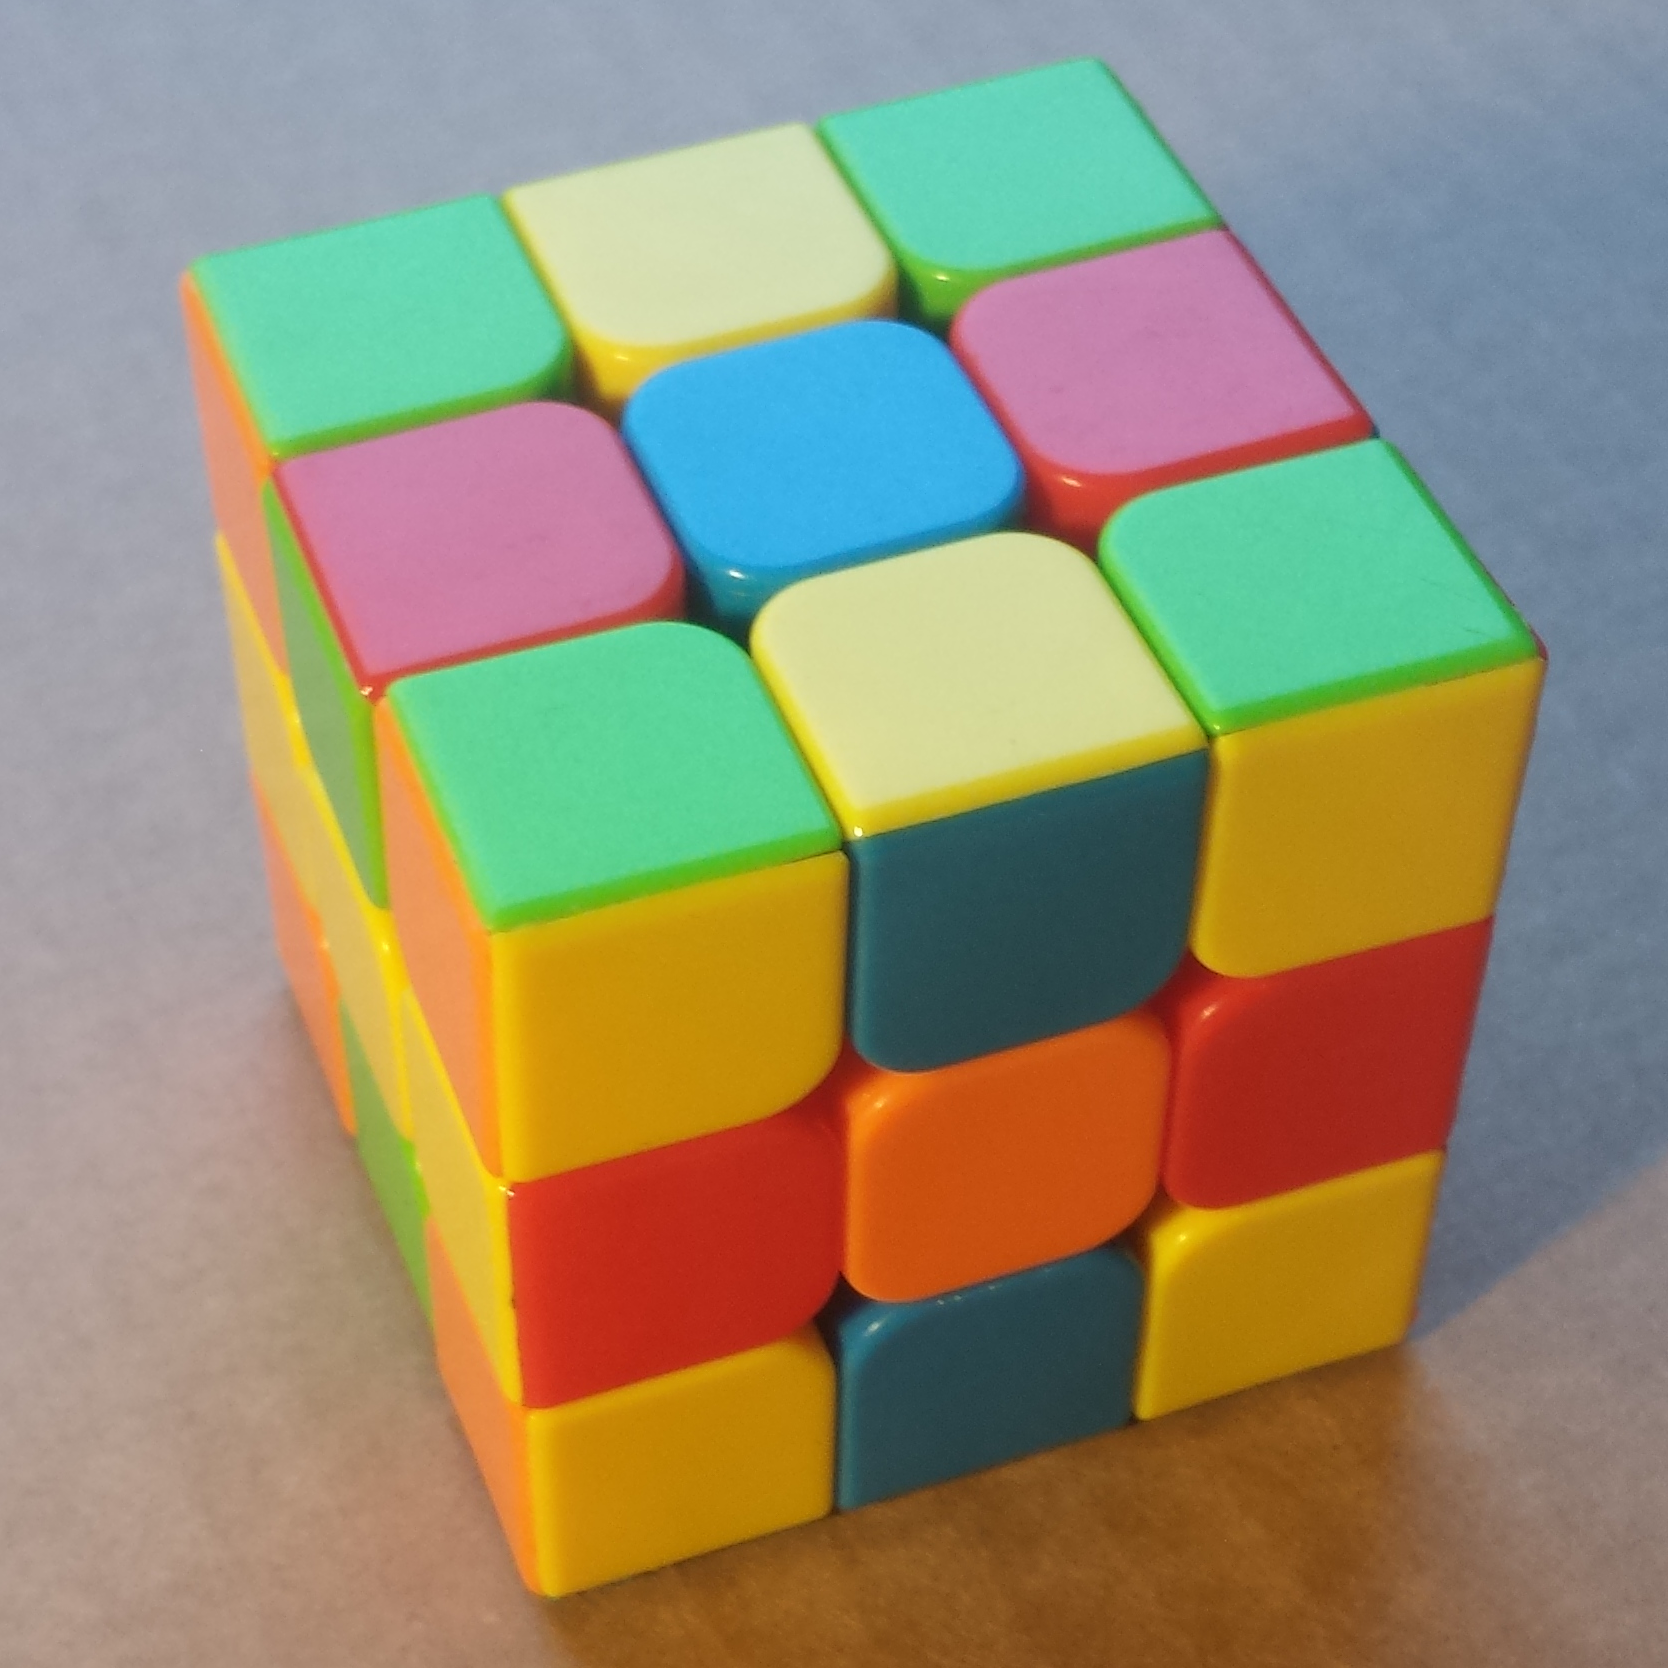
\includegraphics[width=5cm]{origin.jpg}
      \Large{$ \xrightarrow{\mathbf{F}_{g}} $}
      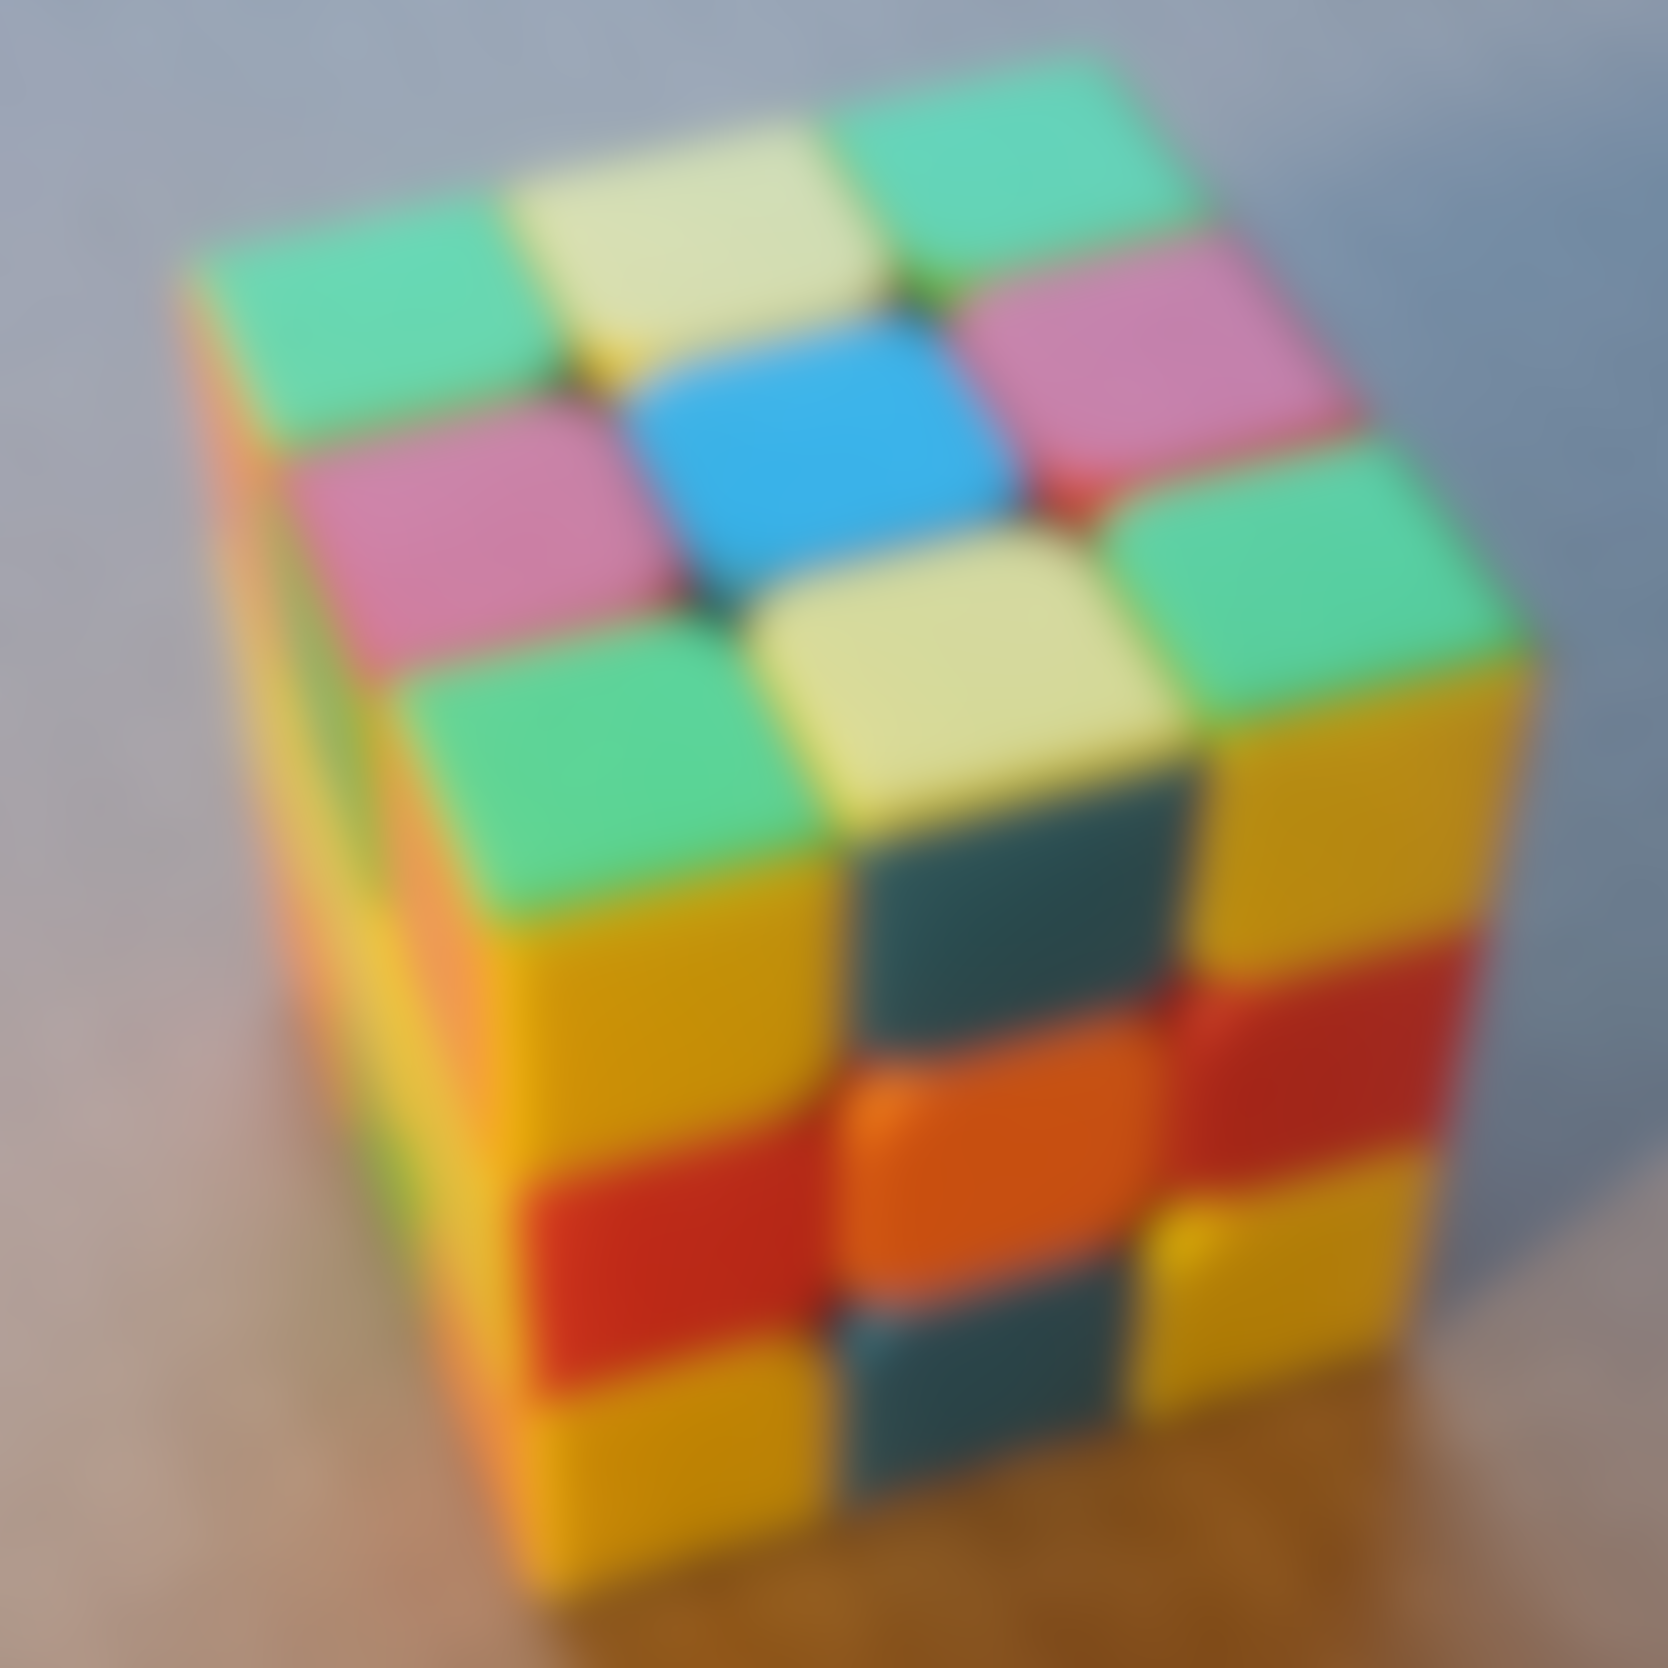
\includegraphics[width=5cm]{Gauss_blur.jpg}
      \caption{Obraz przed i po rozmyciu Gaussa}
      \label {fig:gauss_blur}
   \end{figure}

   Utworzenie przestrzeni skal w algorytmie \textbf{SIFT} polega na stworzemiu rodziny skal $v$ poprzez kilkukreotne skalowenie obrazu wejściowego, a następnie kilkukrotnej filtracji każdej skali $\delta$ z róźnym parametrem rozmycia $\sigma$,
   Standardowo krok skalowania wynosi $ S = 2 \: (M_{n+1} = M_{n} / 2)$, liczba skal wynosi $ n_{\delta} = 3$, a liczba poziomów rozmycia $ n_{\sigma} = 4$

\subsection{Róźnica filtrów Gaussa}:
   Funkcja \textbf{DoG} (Difference of Gaussians - Róźnica filtrów Gaussa) wyznacza obszary na obrazie, które mogą zawierać elementy kluczowe (krok 2 transformacji \textbf{SIFT}). Funkcja \textbf{DoG} jest przybliżeniem \textbf{LoG} (Laplasjan filtru Gaussa) - funkcją filtrują, która pozwala wykryć krawędzie. Filtracja obrazu (Rysunek \ref{fig:DoG})  wykrywa krawędzie niezależnie od ich skali i obrotu, w taki sposób można odrzucić obszary obrazu, dalsza analiza których jest zbędna. Ponieważ w poprzednim kroku sostała stworzona przestrzeń skal z różnym rozmyciem, transformacja \textbf{DoG} jest obliczana dla każdej kolejnej pary zdjęć w każdym zestawie:
   \begin{equation} \label{eq:DoG}
      \mathbf{DoG}(\mathbf{u}) = \mathbf{G}_{\sigma_n}(\mathbf{u}) - \mathbf{G}_{\sigma_{n+1}}(\mathbf{u})
   \end{equation}

   \begin{figure}[h]
      \centering
      \includegraphics[width=6cm]{SIFT_cube_points.png}
      \label {fig:G2DoG}
      \caption{Schemat stosowania przekształcenia DoG dla przestrzeni skal}
      \label {fig:DoGT}
   \end{figure}

   \begin{figure}[h]
      \centering
      \subfloat[Oryginał]{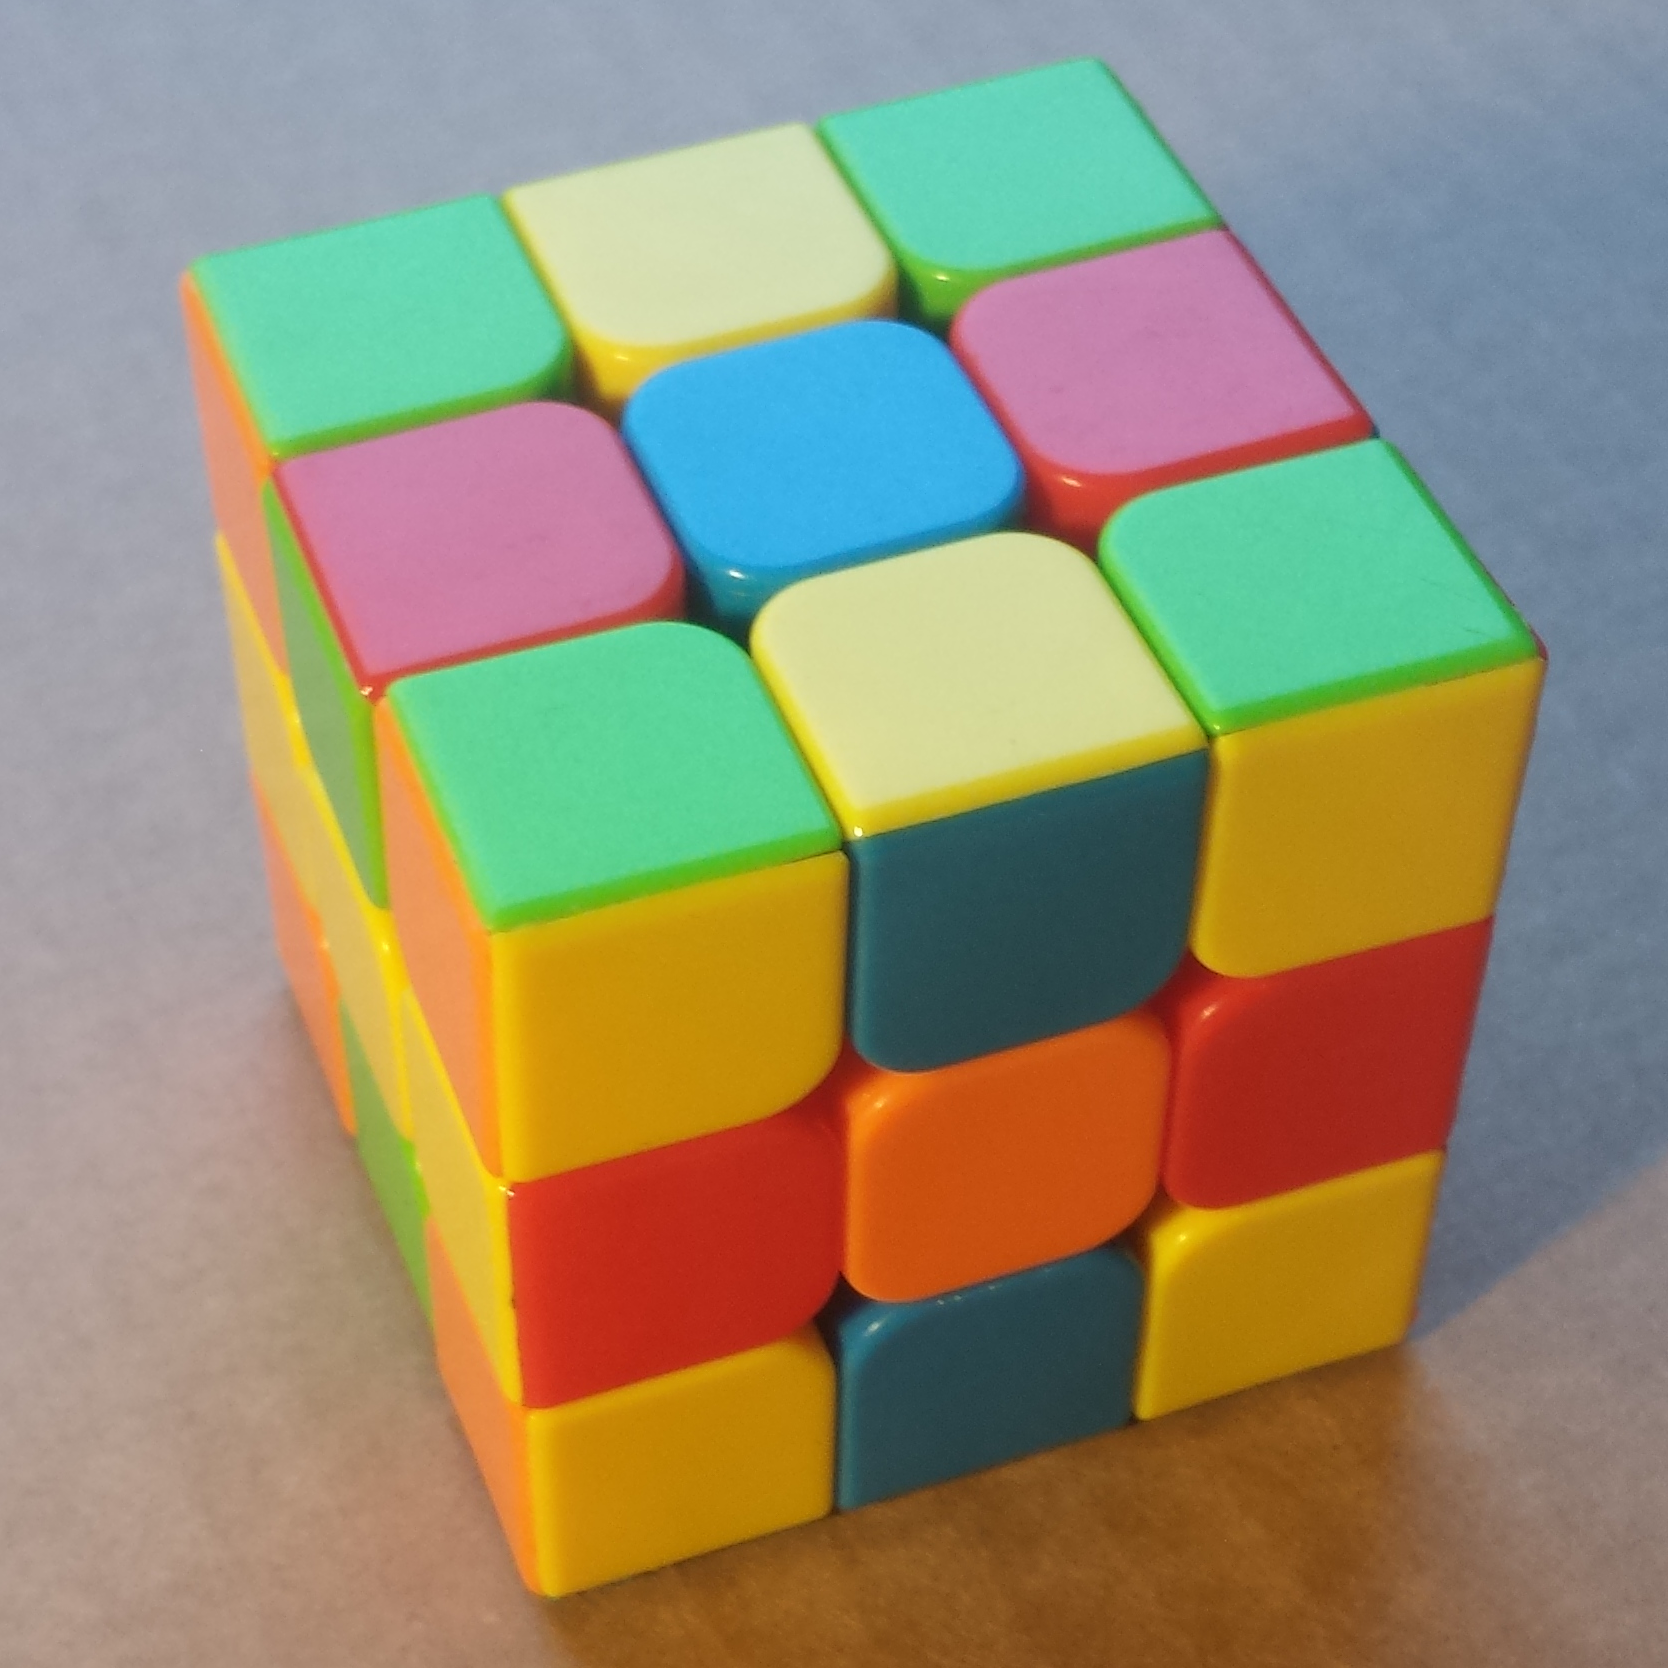
\includegraphics[width=5cm]{origin.jpg}}
      \smallskip{ }
      \subfloat[$\sigma_1 = 1, \sigma_2 = 4$]{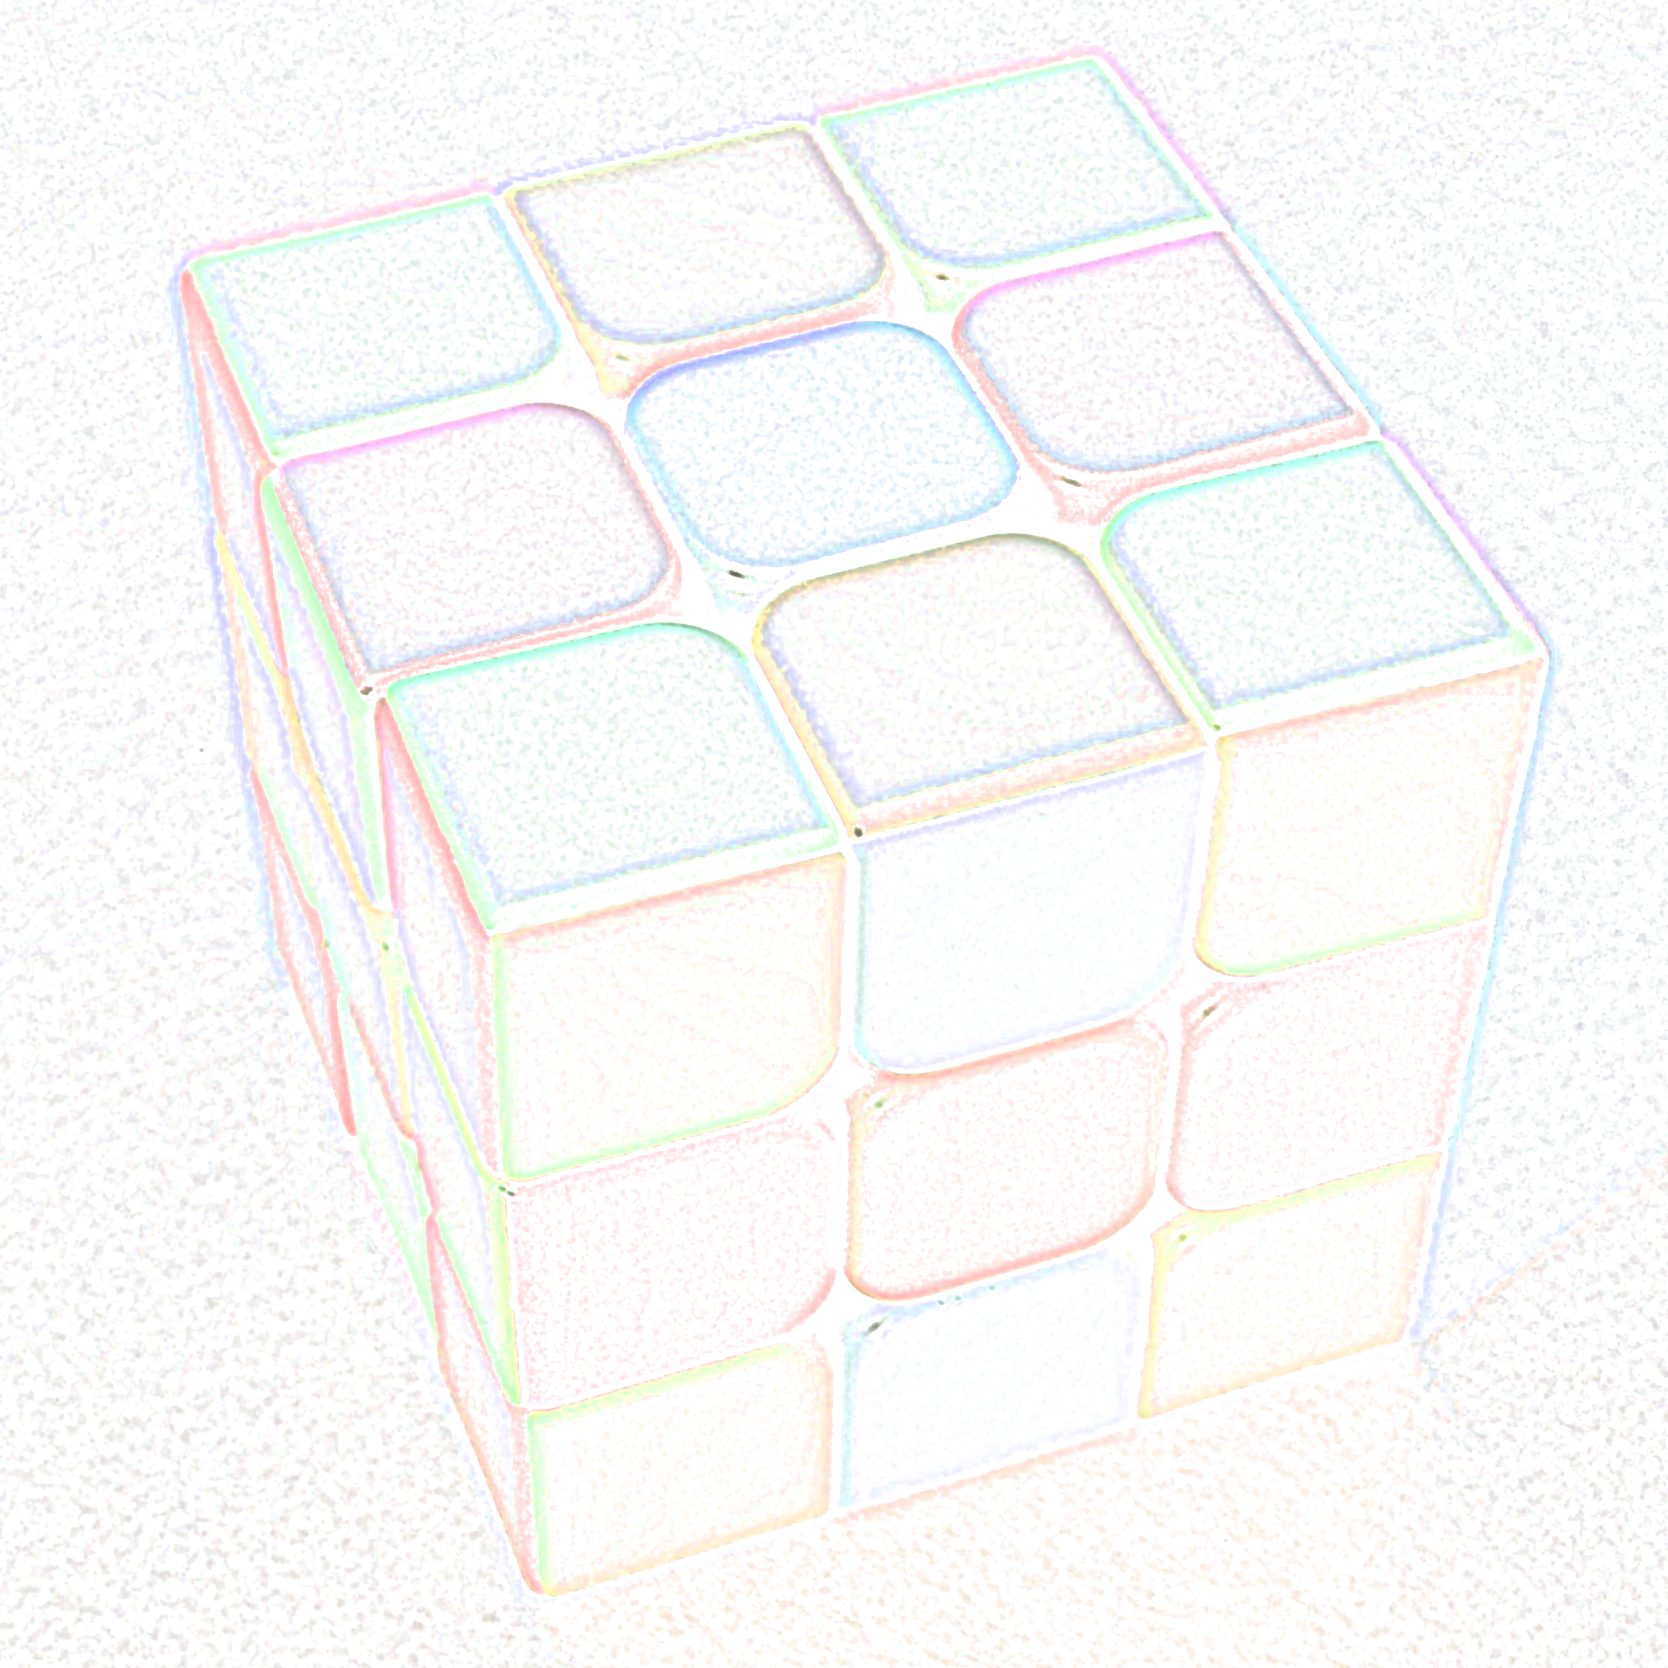
\includegraphics[width=5cm]{DoG_1to4_white.jpg}}
      \smallskip{ }
      \subfloat[$\sigma_1 = 2, \sigma_2 = 16$]{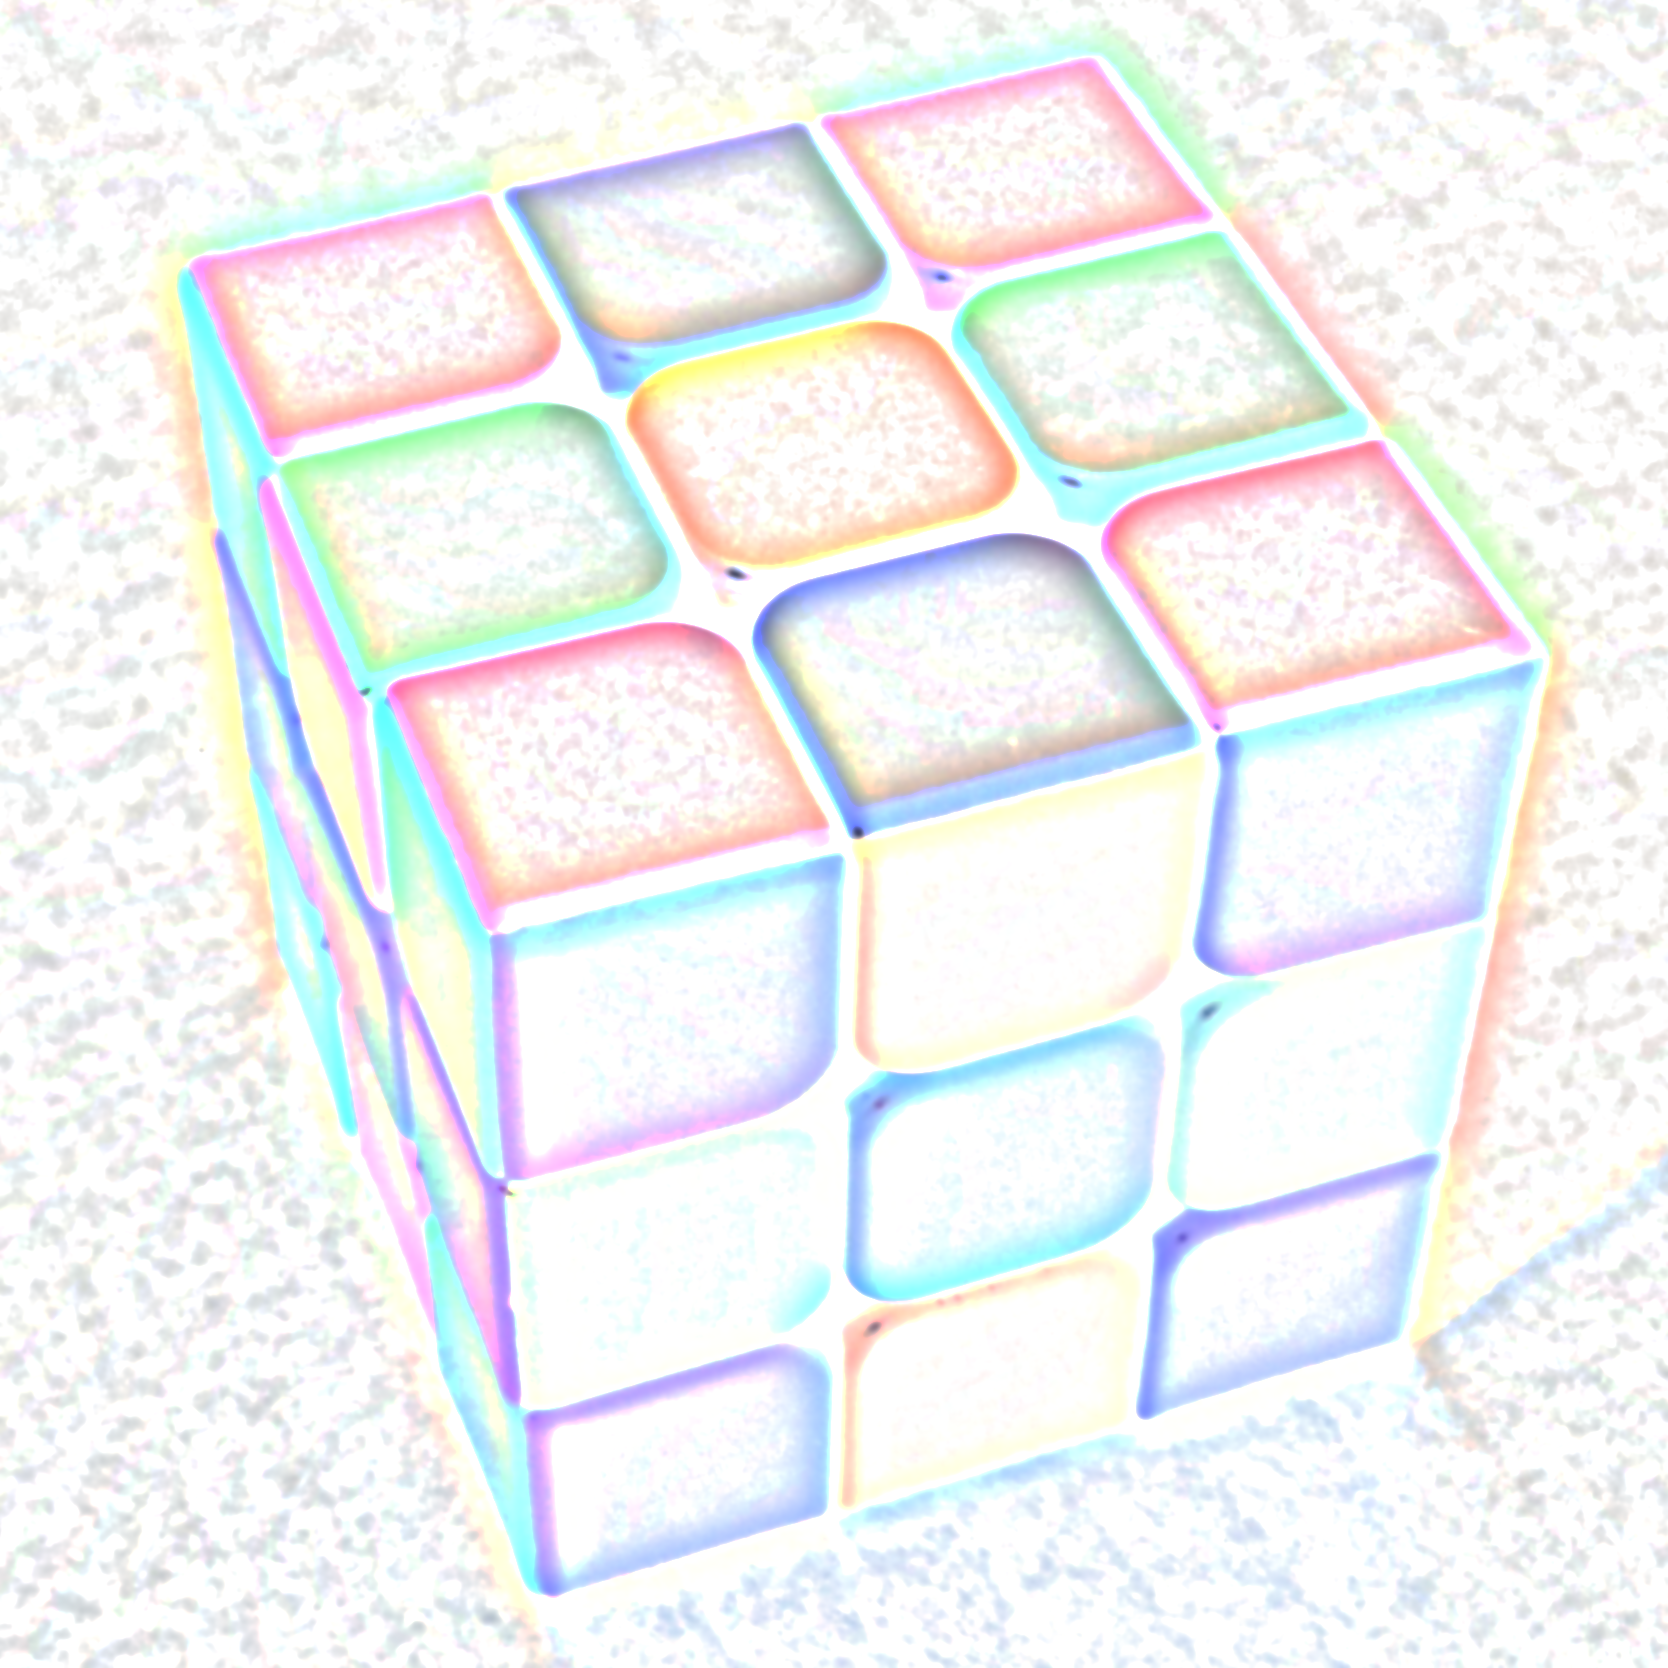
\includegraphics[width=5cm]{DoG_2to16_white.jpg}}
   \caption{Obraz przed i po filtracji DoG}
   \label {fig:DoG}
   \end{figure}

\iffalse

\subsection{Lokalizacja punktów kluczowych. Filtracja}
   Lokalizacja punktów kluczowych polega na wyznaczaniu wyznaczeniu ekstremów wyniku transformacji \textbf{DoG} zdokładnością subpikselową.

   Filtracją punktów polega na wyznaczeniu

\subsection{Przydział obrotu}
      Dla każdego punktu kluczowego jest przydzielana jedna lub więcej orientacji.
      Przekształcenie elementu charakterystycznego w stosunku do lokalizacji, skali i orientacji pozwala zapewnić niezmienność transformacji cechy dla następnych operacji.
      \begin{figure}[h]
         \centering
         \includegraphics[width=6cm]{SIFT_opencv.jpg}
         \label {fig:SIFT_rot}
         \caption{Przydzielony obrót cech na zdjęciu}
      \end{figure}
\subsection{Deskryptor punktu kluczowego}
      Deskryptor cechy jest otrzymany w sposób zastosowania transformata gradientów lokalnych na obszczarze cechy a następnie
      \begin{figure}[h]
         \centering
         \includegraphics[width=8cm]{SIFT_vectors.jpg}
         \label {fig:SIFT_desc}
         \caption{Opis cechy na zdjęciu}
      \end{figure}

      \begin{figure}[h]
         \centering
         \includegraphics[width=5cm]{SIFT_cube_points.jpg}
         \label {fig:SIFT_points}
         \caption{Zlokalizowane cechy na zdjęciu}
      \end{figure}

Cechy zdjęcia wykryte transformacją \textbf{SIFT} są bardzo charakterystyczne, co pozwala z wysokim prawdopodobieństwem wykryć właściwy punkt w bazie danych innego zdjęcia.

\section{Parowanie obrazów}
Ten krok ma 2 cele:
Aby zredukować ilość błędnych par punktów charakterystycznych, kiedy 2 obrazy nie posiadają wspólnych części sceny.
Aby przyspieszyć wykonanie następnego kroku --- \textbf{zestawienie punktów kluczowych}.

\section{Zestawienie punktów kluczowych}

\section{Wyznaczanie kształtów sceny i kokalizacja kamery}
Podejście AdaptiveStructurefromMotion (Rysunek \ref{fig:SfM})

\begin{figure}[h]
   \centering
   \includegraphics[width=7cm]{SfM.png}
   \label {fig:SfM}
   \caption{Wyznaczanie pozycji cechy i ujęcia}
\end{figure}

\fi
